\documentclass[conference]{IEEEtran}
\IEEEoverridecommandlockouts

\usepackage{cite}
\usepackage{amsmath,amssymb,amsfonts}
\usepackage{graphicx}
\usepackage{textcomp}
\usepackage{xcolor}
\usepackage{booktabs}
\usepackage{hyperref}
\usepackage{float}
\usepackage[T1]{fontenc}
\renewcommand{\ttdefault}{cmtt}

\graphicspath{{figures/}}

\begin{document}

\title{Traffic Crash Severity Prediction in San Jose}

\author{
  \IEEEauthorblockN{Eugene Lacatis, Rosnita Dey, Peter Conant, Faye Yang}
  \IEEEauthorblockA{
    \textit{Master's in Software Engineering} \\
    \textit{San Jose State University} \\
    San Jose, United States
  }
}

\maketitle

\begin{abstract}
We merged crash and vehicle records from the San Jose Police Department (SJPD) with highway crash data from the California Highway Patrol's SWITRS system to build a dataset of over 269,000 traffic incidents spanning 2011 through 2024. We predicted crash injury severity on a five-class scale (0 = no injury, 4 = fatal) using features observable at or before the time of the crash: location, weather, time of day, collision type, and driver sobriety. We tested Naive Bayes and Random Forest, finding that Random Forest reached 64\% accuracy with a macro F1 of 0.326. Geographic location and time of day drove most of the model's predictive signal. We also built a Streamlit web app that lets planners and residents explore crash hotspots across San Jose on an interactive map.
\end{abstract}

\begin{IEEEkeywords}
Traffic Crash Severity, Data Mining, Random Forest, Naive Bayes, Class Imbalance, San Jose, SWITRS, SJPD, Geospatial Analysis, Feature Engineering, Streamlit
\end{IEEEkeywords}

% -------------------------------------------------------
\section{Introduction}
% -------------------------------------------------------

San Jose has gotten safer in one sense: total crashes dropped 53\% since 2011. In another sense it has gotten more dangerous, with fatal crash rates rising 43\% over the same window. Fewer crashes, but the ones that do happen are more likely to kill someone. That gap is what motivated this project.

Standard crash analysis focuses on volume: where do the most crashes happen? That question misses low-frequency, high-fatality locations where a handful of crashes produce a disproportionate body count. A model that estimates severity, not just likelihood, gives planners a more honest basis for deciding where to spend a safety budget.

We had three questions going in: which features actually predict crash severity in San Jose; whether Naive Bayes or Random Forest was better suited to this specific problem; and whether we could build something non-technical users could actually use to explore the data. We built a merged SJPD and SWITRS dataset, ran both models, and shipped a Streamlit map application. The sections below document what we found and where the approach still falls short.

% -------------------------------------------------------
\section{Data Collection and Merging}
% -------------------------------------------------------

\subsection{SJPD City Data}

Our primary source was the City of San Jose's Open Data Portal (\texttt{data.sanjoseca.gov}), which publishes SJPD crash and vehicle records going back to 2011. The data comes in two time slices, 2011 to 2021 and 2022 to present, each with a crash table and a vehicle table, so four CSV files total.

The crash table (74,195 records, 33 fields) has location, weather, road surface, lighting, collision type, traffic control, and a severity value. The vehicle table (152,731 records, 27 fields) has driver age, sex, and sobriety; vehicle type and make; safety equipment; and violation codes. We joined them on the \texttt{CrashName} key, one crash linking to multiple vehicles, with an average of 2.06 vehicles per incident (max 14).

Two things are worth knowing about the data across time periods: the 2022-and-later records add \texttt{SpeedingFlag} and \texttt{HitAndRunFlag}, which don't exist in the older files. Driver race and vehicle make/model fields are also about 99\% null in the 2011 to 2021 slice, so they weren't usable.

\subsection{CHP/SWITRS Highway Data}

SJPD covers city streets well but barely touches the freeways. Less than 0.2\% of SJPD records involve highway locations, which means crashes on I-280, I-880, US-101, and SR-87 are mostly absent from the city data. We pulled Santa Clara County crash records from SWITRS (the CHP's statewide system) for 2016 through 2024 to fill that gap. The integration script (\texttt{scripts/integrate\_highway\_data.py}) handled field mapping, geographic filtering, and severity normalization.

SWITRS doesn't give us the same per-party injury severity granularity as SJPD. Highway severity labels end up binary, either no injury or fatal. We can't reliably assign minor, moderate, or severe to highway records, which limits SWITRS data to geographic analysis. All multiclass modeling uses SJPD-only records.

\subsection{Deduplication and Final Dataset}

Since SJPD and CHP both log crashes near city boundaries, some incidents appear in both datasets. We matched on rounded lat/lon (roughly 111-meter precision) and crash date, which flagged 59 SJPD records as likely duplicates and removed them. The final dataset has 269,213 records with a \texttt{data\_source} column indicating origin. For modeling, we use the 152,731 SJPD-only records that have full five-class severity labels.

% -------------------------------------------------------
\section{Exploratory Data Analysis}
% -------------------------------------------------------

\subsection{Target Variable Distribution}

The injury severity target is a five-class ordinal variable. Table~\ref{tab:severity} shows the class distribution. See also Fig.~\ref{fig:target_dist} in the Appendix.

\begin{table}[H]
  \centering
  \caption{Injury Severity Class Distribution (SJPD dataset)}
  \label{tab:severity}
  \begin{tabular}{@{}clrr@{}}
    \toprule
    Class & Label & Count & Share (\%) \\
    \midrule
    0 & No Injury & 41,579 & 56.0 \\
    1 & Minor & 20,011 & 27.0 \\
    2 & Moderate & 9,658 & 13.0 \\
    3 & Severe & 2,293 & 3.1 \\
    4 & Fatal & 654 & 0.88 \\
    \bottomrule
  \end{tabular}
\end{table}

The class imbalance is 63.6:1 between No Injury and Fatal. A model that always guesses ``No Injury'' hits 56\% accuracy without learning anything useful, which makes accuracy a misleading metric here. We used macro F1 and minority-class recall instead.

\subsection{Temporal Patterns}

Crashes peak at 5 PM on Fridays, which is expected from rush-hour traffic. The more useful pattern is at the other end of the clock: late-night crashes (midnight to 4 AM) are a small fraction of total volume but a much higher fraction of serious injuries. That makes time-of-day features matter for severity prediction even when they don't predict crash frequency the same way. See Fig.~\ref{fig:temporal} in the Appendix.

\subsection{Feature Associations with Severity}

We used Cramer's V to measure how strongly each categorical feature associated with severity (Fig.~\ref{fig:cramersv} in the Appendix). Table~\ref{tab:cramersv} shows the top results.

\begin{table}[H]
  \centering
  \caption{Cramer's V Associations with Injury Severity}
  \label{tab:cramersv}
  \begin{tabular}{@{}lll@{}}
    \toprule
    Feature & Cramer's V & Strength \\
    \midrule
    CollisionType & 0.31 & Strong \\
    PrimaryCollisionFactor & 0.28 & Moderate-strong \\
    Sobriety & 0.24 & Moderate \\
    Lighting & 0.22 & Moderate \\
    Weather & 0.19 & Moderate \\
    \bottomrule
  \end{tabular}
\end{table}

CollisionType is the strongest categorical predictor: head-on and pedestrian crashes are in a different severity category than rear-ends and sideswipes. Sobriety shows a clear gradient from sober to under-influence. None of these associations are strong enough to predict severity on their own, but they're consistent with what you'd expect from domain knowledge.

\subsection{Geographic Clustering}

Crashes cluster on Tully Road, Story Road, Capitol Expressway, and the downtown core, and severe crashes cluster even more tightly around high-speed arterials and freeway ramps. That concentration is why location ends up dominating the Random Forest model. See Fig.~\ref{fig:spatial} in the Appendix.

\subsection{Missing Values}

Three fields have high null rates: \texttt{Comment} (89.4\%, excluded), \texttt{HitAndRunFlag} (82.5\%, 2022+ only), and \texttt{SpeedingFlag} (82.5\%, 2022+ only). Everything else used in modeling was below 2\% null. We filled missing categoricals with the string ``unknown'' and dropped records with no coordinates (fewer than 0.1\% of total).

% -------------------------------------------------------
\section{Feature Engineering}
% -------------------------------------------------------

\subsection{Time Features}

We pulled hour, day of week, and month from the timestamp, then added cyclical encodings for hour (\texttt{hour\_sin}/\texttt{hour\_cos}) because standard integer encoding treats midnight and 11 PM as far apart when they're adjacent on the clock. Binary flags for rush hour, weekends, and late night round out the time features.

\subsection{Target Encoding and Train/Test Split}

The five-class severity target (0 to 4) is used as-is. We applied a stratified 80/20 split to preserve class distribution in both sets. Without stratification, the Fatal class (654 records total) could easily end up underrepresented in the test set.

\subsection{Categorical Encoding}

Label encoding for all categoricals (CollisionType, PrimaryCollisionFactor, Weather, Lighting, RoadwaySurface, RoadwayCondition, Sobriety). One-hot encoding would have worked but some fields have high cardinality, and the extra dimensions weren't worth it for tree-based models.

\subsection{Coordinate Normalization}

Latitude and longitude are min-max normalized to [0, 1] to keep scales consistent across features.

% -------------------------------------------------------
\section{Models and Results}
% -------------------------------------------------------

\subsection{Naive Bayes}

We ran Naive Bayes as a deliberate stress test. It has clear theoretical weaknesses on this kind of data, and we wanted to be explicit about why, not just observe that it underperformed, but trace where the assumptions break.

\begin{table}[H]
  \centering
  \caption{Naive Bayes vs. Random Forest Performance}
  \label{tab:results}
  \begin{tabular}{@{}llll@{}}
    \toprule
    Model & Macro F1 & Sev+Fatal Recall & Notes \\
    \midrule
    GaussianNB & 0.278 & 0.051 & All features \\
    CategoricalNB & 0.359 & 0.097 & Categorical only \\
    Random Forest & 0.326 & 0.058 & All features, balanced \\
    \bottomrule
  \end{tabular}
\end{table}

The independence assumption breaks first. Sobriety and lighting are correlated, since drinking crashes spike at night. Weather and road surface are correlated, since wet pavement follows rain. Naive Bayes treats those pairs as independent and introduces systematic bias as a result.

GaussianNB makes things worse by assuming features are normally distributed. Label-encoded categoricals aren't. CollisionType integers (0=broadside, 1=head-on, 2=rear-end) aren't a continuous variable and don't fit a Gaussian. CategoricalNB avoids that problem but creates a new one: it can't accept continuous inputs like latitude and longitude, so it was forced to drop the two most predictive features in the dataset.

Neither variant has a \texttt{class\_weight} parameter, so both learned to predict ``No Injury'' and essentially ignored the minority classes. These aren't just implementation gaps. They reflect a structural mismatch between Naive Bayes assumptions and how crash data actually works.

See Fig.~\ref{fig:confusion} in the Appendix for the confusion matrices across all three models.

\subsection{Random Forest}

Random Forest doesn't have those problems. It handles mixed feature types, doesn't assume independence, and \texttt{class\_weight=`balanced'} makes it account for the imbalance explicitly. We ran 100 trees with normalized coordinates and label-encoded categoricals on a stratified 80/20 split.

Results: 64\% overall accuracy, macro F1 of 0.326, Severe+Fatal recall of 0.058. No Injury precision 72\%, Fatal precision 81\%, Fatal recall 21\%.

Top feature importances: Latitude (0.239), Longitude (0.233), Hour (0.115), CollisionType (0.111), Day of Week (0.082). Latitude and longitude together account for 47\% of total importance. The model mostly learned where and when bad crashes tend to happen.

\noindent\fbox{\parbox{\columnwidth}{%
\textbf{[PLACEHOLDER, Classification Report]:} Full per-class precision, recall, and F1 scores for all five severity classes needed here. Extract the complete \texttt{sklearn.metrics.classification\_report} output from \texttt{notebooks/05\_naive\_bayes\_analysis.ipynb} and insert as a table.
}}

\subsection{Discussion}

CategoricalNB's macro F1 (0.359) is technically higher than Random Forest's (0.326), but only because it excluded the hardest-to-use features. A model that can't incorporate location doesn't solve the problem we were working on. Random Forest is the better choice for any application that needs geographic risk estimates.

The bigger issue across all models is minority-class recall. A 63.6:1 imbalance is hard to overcome with \texttt{class\_weight} alone. SMOTE or ensemble resampling is the logical next step, along with gradient boosting methods like XGBoost and LightGBM, which tend to handle imbalanced data better than Random Forest.

The feature importances also raise a question worth flagging: the model is learning geography, not causation. It knows that crashes near a particular interchange tend to be severe. It doesn't know whether adding a traffic light there would change that. Those are different models, and the second one is harder.

% -------------------------------------------------------
\section{Web Application}
% -------------------------------------------------------

The app is built with Streamlit and pydeck, a Python wrapper for the deck.gl WebGL mapping library. It loads from the processed SJPD dataset and deduplicates on startup to one row per unique (Latitude, Longitude, CrashDateTime), which prevents multi-vehicle records from stacking on top of each other in point mode.

\begin{quote}
\texttt{conda activate crash-severity} \\
\texttt{streamlit run webapp/app.py}
\end{quote}

Point mode shows individual crashes as colored dots sized and colored by severity. Click one to see date, time, severity label, collision type, weather, lighting, road surface, injury counts, and speeding/hit-and-run flags where available. Heatmap mode uses density weighting across the full 269K records to show where crashes concentrate, which is more useful than point mode for spotting corridors at city scale. A sidebar filter cuts the display to selected severity classes.

% -------------------------------------------------------
\section{Conclusion}
% -------------------------------------------------------

San Jose crash severity is predictable, but only in a particular sense. The model knows where and when bad crashes happen. It doesn't know why, and it can't tell you whether a specific infrastructure change would shift the odds. That distinction matters for anyone hoping to use this for policy.

Naive Bayes was the wrong tool for this data: too many violated assumptions, no way to handle class imbalance, and for the categorical variant, no path to including location at all. Random Forest handled the problem better and confirmed that geographic clustering is real and strong, but 64\% accuracy with a macro F1 of 0.326 and poor minority-class recall leaves significant room to improve.

The most productive next directions are SMOTE or similar resampling to address the 63.6:1 imbalance, gradient boosting models, and causal models that separate where crashes are severe from what makes them severe, for anyone interested in policy applications rather than visualization.

% -------------------------------------------------------
\section*{Acknowledgment}
% -------------------------------------------------------

Thanks to Prof. Jung Suh, CMPE 255 Data Mining, San Jose State University, for guidance throughout the semester. The SJPD crash dataset is maintained by the City of San Jose Open Data Team; the SWITRS data comes from the California Highway Patrol. We used scikit-learn, Streamlit, pydeck, pandas, and matplotlib throughout.

% -------------------------------------------------------
\appendix
\section{Figures}
% -------------------------------------------------------

\begin{figure*}[h]
  \centering
  
\includegraphics[width=\textwidth]{target_distribution.png}
  \caption{Injury severity distribution: class counts (left) and share by class (right).}
  \label{fig:target_dist}
\end{figure*}

\begin{figure*}[h]
  \centering
  
\includegraphics[width=\textwidth]{temporal_patterns.png}
  \caption{Temporal patterns: crash counts by year, month, day of week, and hour of day.}
  \label{fig:temporal}
\end{figure*}

\begin{figure*}[h]
  \centering
  
\includegraphics[width=\textwidth]{feature_associations.png}
  \caption{Cramer's V associations between categorical features and injury severity (top 10 features).}
  \label{fig:cramersv}
\end{figure*}

\begin{figure*}[h]
  \centering
  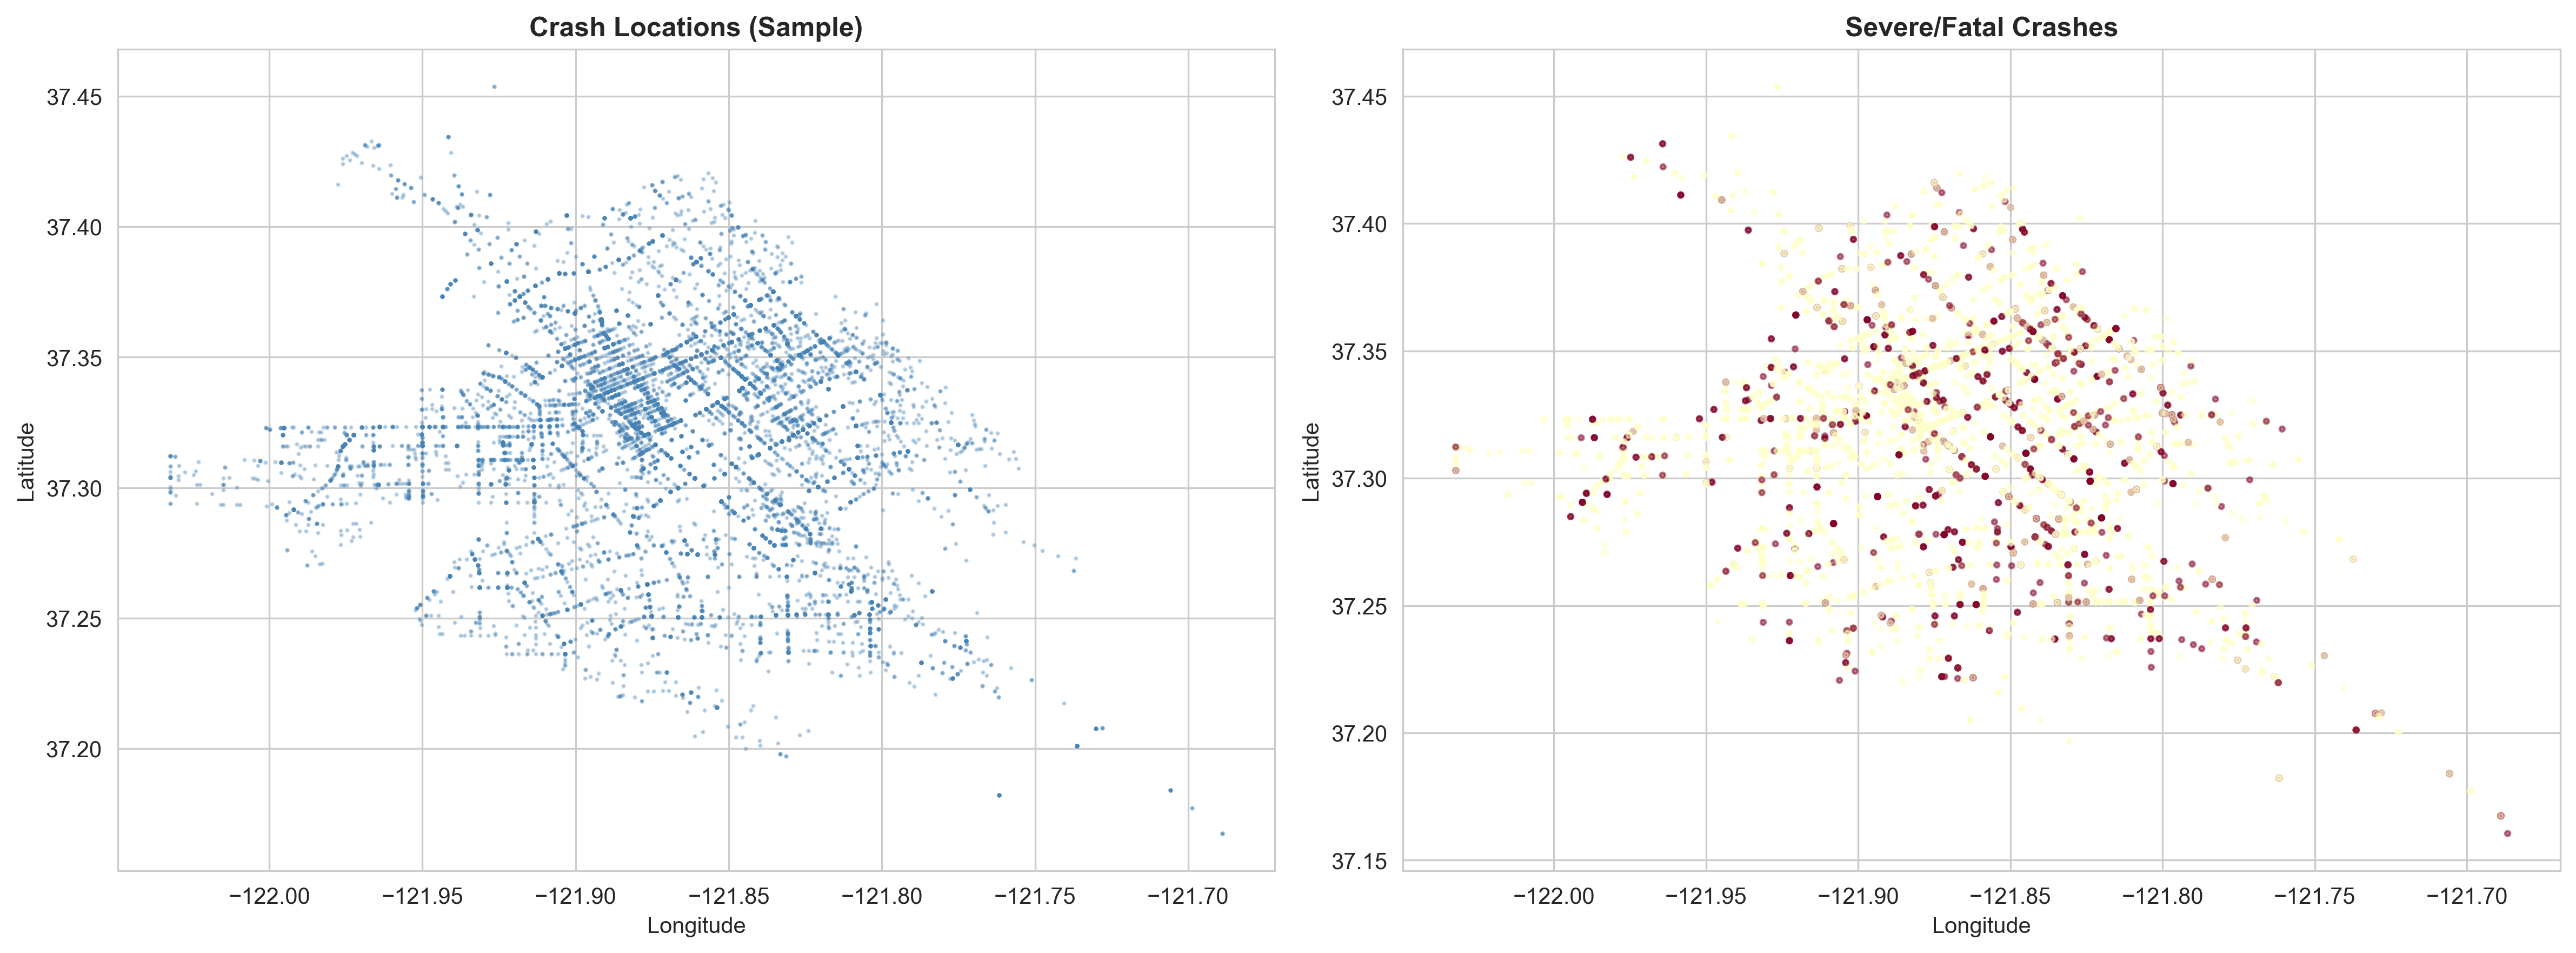
\includegraphics[width=\textwidth]{spatial_distribution.png}
  \caption{Spatial distribution of crashes across San Jose, 2011 to 2024.}
  \label{fig:spatial}
\end{figure*}

\begin{figure*}[h]
  \centering
  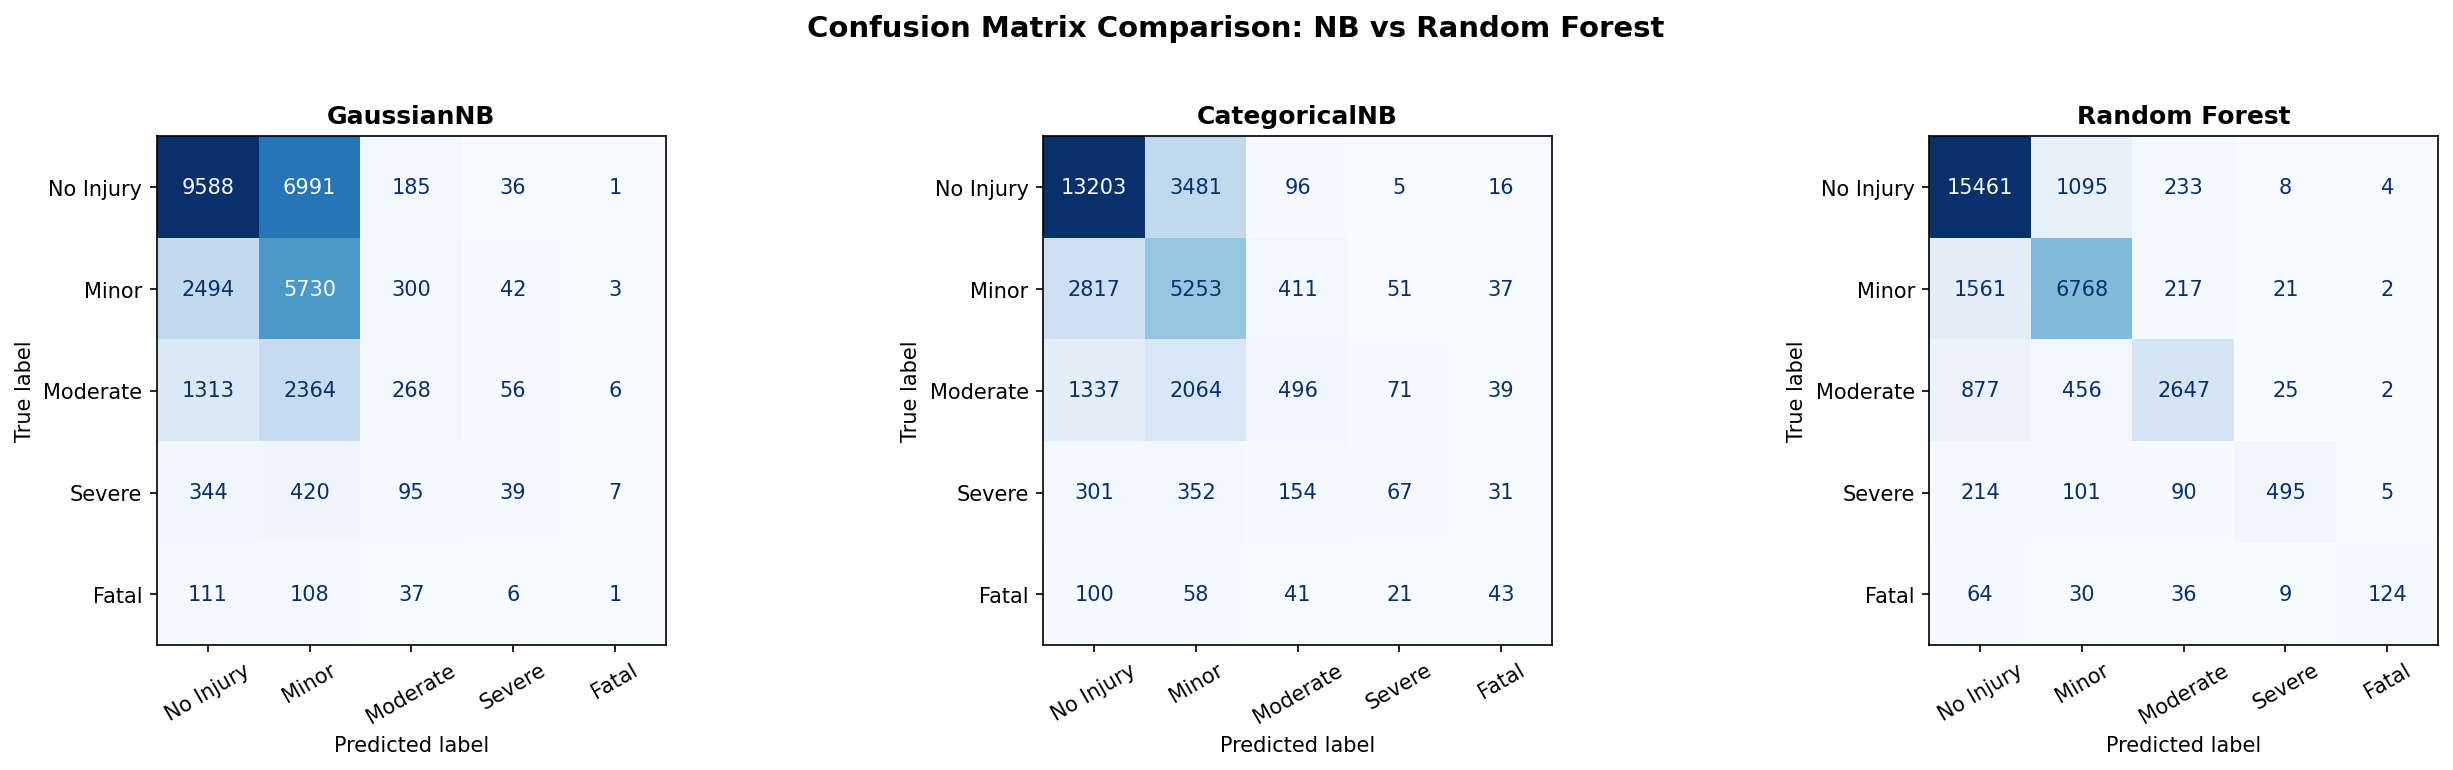
\includegraphics[width=\textwidth]{nb_vs_rf_confusion_matrices.png}
  \caption{Confusion matrices for GaussianNB (left), CategoricalNB (center), and Random Forest (right) on the held-out test set.}
  \label{fig:confusion}
\end{figure*}

\begin{figure*}[h]
  \centering
  
\includegraphics[width=\textwidth]{severity_by_collisiontype.png}
  \caption{Injury severity distribution by collision type.}
  \label{fig:sev_collision}
\end{figure*}

\begin{figure*}[h]
  \centering
  
\includegraphics[width=\textwidth]{severity_by_sobriety.png}
  \caption{Injury severity distribution by driver sobriety status.}
  \label{fig:sev_sobriety}
\end{figure*}

\begin{figure*}[h]
  \centering
  
\includegraphics[width=\textwidth]{severity_temporal.png}
  \caption{Injury severity by hour of day and day of week (stacked bar charts).}
  \label{fig:sev_temporal}
\end{figure*}

\end{document}
